\section*{Blatt 2}

\subsection*{2.1 - Cache-Kohärenz}

\subsubsection*{a) Cachegröße}

\texttt{0x10} ist hexadezimal für 16. Wenn der Cache Agent für eine Adresse $x$ nun $x$ durch 16 teilt, erhält er die Adresse der Cachezeile, in der $x$ liegt. 

\subsection*{2.2 - Datenlayout}

\subsubsection*{a) Datenlayout der Partikel}

In Abbildung \ref{fig:data_layout} sind die ersten drei Partikel abgebildet. Jedes Element besteht aus aus 8 Datenelementen mit jeweils 4 Byte Größe. Die Cachezeilengröße beträgt 64 Byte, somit passen genau zwei Elemente in eine Cachezeile. Diese Grenze ist in rot eingezeichnet.

\begin{figure}[H]
  \centering
  \makebox[\linewidth][c]{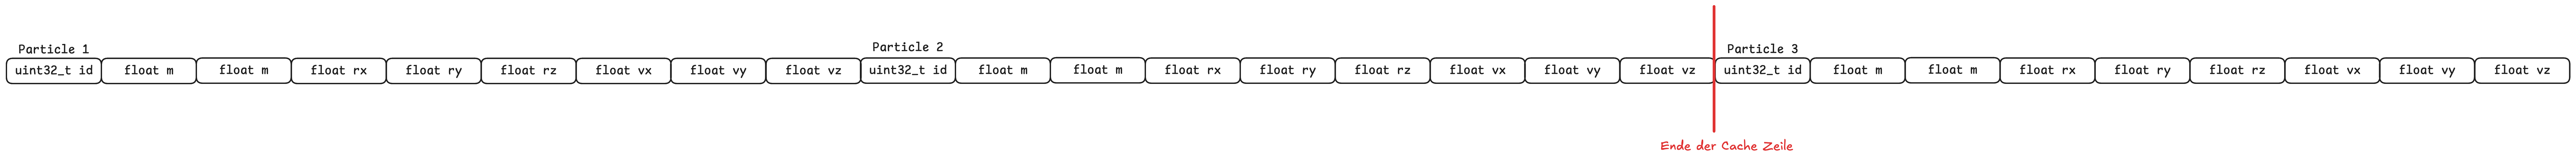
\includegraphics[width=0.9\paperwidth]{Images/ex2-2-Layout.png}}
  \caption{Datenlayout der ersten drei Partikel}
  \label{fig:data_layout}
\end{figure}

\subsubsection*{b) Cache Misses}

Für jede Berechnung sind die 32 Byte eines Partikels notwendig und der Zeitunterschied $dt$. Laut Annahme der Aufgabenstellung beginnt jede $\texttt{calloc}$ Speicherreservierung immer an der Grenze einer Cachezeile. Deswegen muss $dt$ in einer anderen Cachezeile vorhanden sein. Des weiteren gehen wir davon aus, dass $dt$ für alle Berechnungen gleich ist.

Sei $n$ die Anzahl an Kernen, auf die die Berechnung aufgeteilt wird. Jeder Kern braucht Zugriff auf $dt$. Da beim ersten Zugriff $dt$ noch nicht im Cache vorhanden ist, wird für jeden Kern ein Cache Miss verzeichnet, da $dt$ initial geladen werden muss. Dafür muss gelten, dass $dt$ während eines Berechnungschrittes konstant bleibt.

Beim Laden einer Cachezeile werden 2 Partikel geladen, da eine Cachezeile genau zwei Partikel enthält. So erhalten wir bei jedem zweiten Zugriff auf einen Partikel einen Cache Hit.

Zusammen können wir also die Formel

$$
\text{CacheMisses} = \frac{1000000}{2} + n
$$

Diese Formel gilt allgemein für beliebige $n \geq 1$. Da die Aufgabenstellung von einem einzelnen Prozessor ausgeht ($n = 1$), ergibt sich ein konkreter Wert von $\frac{1000000}{2} + 1 = 500001$ Cache Misses. Die Verdrängungsstrategie des Caches wird weder hier noch in der Vorlesung beschrieben. Gelten muss aber, dass die Cachezeile mit $dt$ nicht verdrängt wird, da sonst bei jedem Zugriff auf einen Partikel ein Cache Miss verzeichnet werden würde. Es muss also eine Verdrängungsstrategie vorliegen, die $dt$ im Cache hält, solange die Berechnung läuft. Die bereits benutzten Partikel können verdrängt werden, da sie nicht mehr benötigt werden.

\subsubsection*{c) Cache Misses mit 5 Arrays}
\label{sec:cache-misses-arrays}

Der einstufige Cache des Kerns beträgt 256 KBytes = 262.144 Bytes. Jede Cache Zeile ist 64 Byte groß, somit können 32.768 Cachezeilen im Cache gehalten werden. Eine davon muss die Cachezeile mit $dt$ sein, da sonst bei jedem Zugriff auf einen Partikel ein Cache Miss verzeichnet werden würde. 
Um $\overrightarrow{r} \leftarrow \overrightarrow{r} + \overrightarrow{v} \cdot dt$ zu berechnen müssen folgende Zugriffe gemacht werden:

Wir müssen insgesamt 6 Arrays laden, nämlich $\overrightarrow{r_x}$, $\overrightarrow{r_y}$, $\overrightarrow{r_z}$, $\overrightarrow{v_x}$, $\overrightarrow{v_y}$ und $\overrightarrow{v_z}$. Wir müssen die Arrays mit den Ids und Massen nicht laden, da diese nicht für die Berechnung notwendig sind. Jeder Zugriff auf ein Array führt zu einem Cache Miss, jedoch werden bei jedem Zugriff 16 weitere Elemente geladen, da in in den 64 Byte der Cachzeile $\frac{64}{4} = 16$ Elemente passen. Somit erhalten wir bei jedem 17. Zugriff auf ein Array einen Cache Miss, da die vorherigen 16 Elemente bereits im Cache sind. Es gilt also:

$$
\text{CacheMisses} = 6 \cdot \frac{1.000.000}{16} + 1 = 375.001
$$

Im Vergleich sehen wir als, dass die Anzahl der Cache Misses mit 5 Arrays deutlich geringer ist als mit einem Array, da bei einem Array nur 2 Elemente pro Cachezeile geladen werden, während bei 5 Arrays 16 Elemente pro Cachezeile geladen werden. Somit können wir die Anzahl der Cache Misses um $\frac{500.001 - 375.001}{500.001} \approx 25\%$ reduzieren, was eine deutliche Verbesserung darstellt.

\subsection*{2.3 - Messungen}

Die Berechnungen haben wir auf einem MacBook Pro M2 mit 16 GB RAM durchgeführt. Das Betriebssystem ist macOS 26.4.1 (Darwin 25.4.0) und der Compiler ist Apple clang 21.0.0 (clang-2100.0.123.102), target arm64. Der vollständige Quellcode (\texttt{structures.c}, \texttt{arrays.c}) sowie das \texttt{Makefile} sind im Archiv der Abgabe beigefügt.

Da auf macOS die System-Header (z.B. \texttt{stdint.h}) im Xcode SDK liegen und nicht automatisch gefunden werden,
musste im \texttt{Makefile} der Compiler explizit über \texttt{xcrun} gesetzt und der SDK-Pfad per \texttt{-isysroot}
übergeben werden. Vermutlich liegt dies daran, dass der Nix-Paketmanager eine eigene \texttt{clang}-Version
in den \texttt{PATH} einträgt, welche die macOS-System-Header nicht kennt und den Apple-Compiler verdrängt:

\begin{verbatim}
CC = $(shell xcrun -f clang)
SDK = $(shell xcrun --sdk macosx --show-sdk-path)
CFLAGS = -std=c11 -isysroot $(SDK)
\end{verbatim}

Folgende Messergebnisse haben wir erhalten.

\begin{table}[H]
  \centering
  \begin{tabular}{|l|l|r|r|r|}
    \hline
    \textbf{Programm} & \textbf{Flag} & \textbf{real} & \textbf{user} & \textbf{sys} \\
    \hline
    structures & \texttt{-O0} & 4.004s & 3.565s & 0.029s \\
    structures & \texttt{-O3} & 1.048s & 0.771s & 0.011s \\
    arrays     & \texttt{-O0} & 3.068s & 2.788s & 0.021s \\
    arrays     & \texttt{-O3} & 0.767s & 0.502s & 0.009s \\
    \hline
  \end{tabular}
  \caption{Laufzeitmessungen mit \texttt{-O0} und \texttt{-O3}}
  \label{tab:timing}
\end{table}

Wir können sehen, dass die unoptimierte Varianten (\texttt{-O0}) in beiden Fällen langsamer sind als die Compiler optimierten Varianten (\texttt{-O3}). Genau wie in Aufgabe 2.2c vorhergesagt, ist die Variante mit den Arrays pro Element schneller, da mehr Cache Hits auftreten.

Der Speedup durch \texttt{-O3} ist in beiden Fällen ähnlich (ca. $3.8\times$ bei \texttt{structures}, ca. $4.0\times$ bei \texttt{arrays}). \texttt{-O3} aktiviert unter anderem Function Inlining (der \texttt{calculate}-Aufruf in \texttt{structures} entfällt), Loop Unrolling und bessere Registerzuweisung. Möglicherweise wird der \texttt{arrays}-Loop durch SIMD-Vektorisierung beschleunigt, da die Daten als zusammenhängende Arrays gleichen Typs vorliegen. Beim \texttt{structures}-Programm erschwert das AoS-Layout eine effiziente Vektorisierung über mehrere Partikel.

\subsection*{2.4 - PCAM Matrix Multiplikation}

\subsubsection*{a) PCAM}

Als \textit{Schulmethode} der Matrixmultiplikation nehmen wir $C = A \cdot B$ mit 
$$
c_{ij} = \sum_k a_{ik} \cdot b_{kj}
$$

\paragraph{Step 1 - Partitionierung} Im Rahmen der Lehrveranstaltung konzentrieren wir uns auf quadratische Matrizen. Da keine Matrixeinträge gleich berechnet werden, eigenen diese sich gut als Partitionierung. Die in der Übung vorgestellten Kriterien werden hier erfüllt.
\begin{enumerate}
  \item Die Anzahl der Tasks ist $n^2$ und somit für genügend große $n$ eine Größenordnung höher als die Anzahl der Kerne.
  \item Es tritt keine Redundanz auf, weil jeder Eintrag unterschiedlich berechnet wird.
  \item Die Lastenverteilung ist identisch, da die Berechnungsvorschrift für alle gleich ist.
  \item Die Tasks skalieren adequat (quadratisch) mit der Größe der Matrix.
\end{enumerate}

\paragraph{Step 2 - Communication} Wie in der Übung vorgestellt, können wir die Kommunikation in die folgenden Kategorien einteilen:
\begin{itemize}
    \item \textit{Lokal vs. Global}: Die finale Zusammensetzung der Matrix benötigt die Daten aller anderen Tasks, also ist die Kommunikation global.
    \item \textit{Strukturiert vs. Unstrukturiert}: Die Kommunikation ist struktuiert, weil nur in einem festgelegtem Pattern kommuniziert wird. 
        Alle Tasks geben ihr Ergebnis an die Task weiter, die das Endergebnis berechnet. 
    \item \textit{Statisch vs. Dynamisch}: Die Kommunikation ist statisch, da die Kommunikationspartner bereits vor der Berechnung feststehen und sich nicht ändern.
        \item \textit{Synchron vs. Asynchron}: Die Kommunikation ist für die berechnenden Tasks asynchron, 
            da die Tasks nicht auf die Ergebnisse der anderen Tasks warten müssen, um ihre Berechnung durchzuführen. 
            Die Task, die das Endergebnis berechnet, muss jedoch auf die Ergebnisse aller anderen Tasks warten, 
            bevor sie mit der Berechnung beginnen kann.
\end{itemize}

Wie bereits schon angeschnitten ist das Kommunikationsmuster für das Einsammeln zentralisiert (sternförmig), da alle Tasks ihre Ergebnisse an die Task weitergeben, die das Endergebnis zusammensetzt. Im Shared-Memory-Modell (wie beim SPMD-Ansatz auf Mehrkernprozessoren) entfällt dieses Einsammeln jedoch vollständig: Jede Task schreibt ihr Ergebnis direkt in die entsprechende Position von $C$, da alle Tasks auf denselben Speicher zugreifen.

In der Übung wurden folgende Kriterien für die Kommunikation vorgestellt:
\begin{enumerate}
    \item{\textit{Ausgewogenheit}}: Jede Task führt die gleiche Anzahl an Berechnungen durch, daher ist die Kommunikation ausgewogen.
        Die Task, die das Endergebnis berechnet, hat jedoch eine höhere Kommunikationslast, da sie die Ergebnisse aller anderen Tasks sammeln muss.
        Wir sehen aber keinen sinnvoll Weg, die Kommunikation besser zu verteilen. Es finden eigentlich keine Berechnungen mehr statt,
        denn die Ergebnisse der anderen Tasks müssen nur noch eingesammelt und in $C$ eingetragen werden, was im Vergleich zur Berechnung der Einträge
        von $C$ relativ wenig Aufwand ist.
    \item{\textit{Lokalität}}: Jede berechnende Task kommuniziert mit genau einem Partner (dem Kollektor), was eine gute Lokalität ergibt. Der Kollektor hingegen muss mit allen $n^2$ Tasks kommunizieren, was eine schlechte Lokalität bedeutet.
    \item{\textit{Nebenläufigkeit}}: Alle berechnenden Tasks können vollständig parallel arbeiten, da sie keine gegenseitigen Abhängigkeiten haben. Die Gesamtberechnung ist abgeschlossen, sobald alle $n^2$ Tasks fertig sind.
    \item{\textit{Überlappung}}: Eine Überlappung von Kommunikation und Berechnung ist nicht möglich, da eine Task ihr Ergebnis erst nach Abschluss der Berechnung senden kann. Die Kommunikation findet also ausschließlich nach der Berechnung statt.
\end{enumerate}

\paragraph{Step 3 - Agglomeration} Wir können die Anzahl der Tasks reduzieren, indem wir Zeilen oder Spalten von $C$ als Task definieren. Dadurch erhalten wir $n$ Tasks, die jeweils eine Zeile oder Spalte von $C$ berechnen. 
Die Kommunikation wird dadurch reduziert: statt $n^2$ müssen nur noch $n$ Ergebnisse eingesammelt werden.

Auch hier können wir die Kriterien für die Agglomeration bewerten:
\begin{enumerate}
    \item{\textit{Kommunikationskosten}}: Die Kommunikationskosten sinken, da der Kollektor nun nur noch $n$ statt $n^2$ Nachrichten empfangen muss.
    \item{\textit{Lastenverteilung}}: Die Lastenverteilung bleibt ausgewogen, da jede Task immer noch die gleiche Anzahl an Berechnungen durchführt (jede Task berechnet eine Zeile oder Spalte von $C$).
    \item{\textit{Skalierbarkeit}}: Die Skalierbarkeit bleibt erhalten, da die Anzahl der Tasks immer noch linear mit der Größe der Matrix skaliert. 
    \item{\textit{Nebenläufigkeit}}: Die Nebenläufigkeit bleibt erhalten, da alle Tasks weiterhin parallel arbeiten können.
\end{enumerate}

Die Matrix zeilen- oder spaltenweise zu berechnen, führt zu mehr Cache Hits, da für jede Berechnung entweder der Spalten- oder Zeilenvektor von $A$ bzw. $B$ im Cache gehalten werden kann, während die Einträge von $C$ sequentiell berechnet werden.
Für große Matrizen könnte es jedoch Sinn ergeben, die Spalten oder Zeilen weiter zu partitionieren, um die Anzahl der Tasks zu erhöhen und damit die Parallelität zu verbessern. Die oben beschriebnen Aspekte bleiben aber dennoch fast vollständig erhalten. Nur die Anzahl der Kommunikationspartner des Kollektors erhöht sich, da nun mehr Tasks ihre Ergebnisse an den Kollektor senden müssen. Mehrere Tasks würden aber zu einer schnelleren Berechnung führen, weshalb die erhöhte Kommunikationslast des Kollektors in Kauf genommen werden könnte.


\paragraph{Step 4 - Mapping} Da die Rechenlast pro Task identisch ist und die Anzahl der Tasks statisch feststeht, verwenden wir das \textit{SPMD-Modell} mit statischem Mapping. Jeder agglomerierte Task (eine Zeile von $C$) wird exakt einem Kern zugewiesen.

Für die Topologie-Optimierung passt der \textit{Stern-Ansatz} gut zu unserem Kommunikationsmuster, da alle Tasks ihr Ergebnis an einen zentralen Kollektor senden. Im Shared-Memory-Modell entfällt dies wie bereits erwähnt vollständig.

Da die Rechenlast pro Task identisch ist und die Anzahl der Tasks und Datenmengen statisch feststehen, ist kein komplexer Lastausgleich notwendig.

\subsubsection*{b) Validierung}

Die parallelisierte Berechnung der Matrixmultiplikation funktioniert identisch mit der sequentiellen Berechnung, da die Berechnung jedes Eintrags von $C$ unabhängig von den anderen Einträgen ist. Es gibt also keine Datenabhängigkeiten zwischen den Tasks, die zu Inkonsistenzen führen könnten. Solange die parallele Implementierung korrekt ist (d.h. jeder Task berechnet die richtigen Einträge von $C$ und schreibt sie an die richtige Stelle), wird das Ergebnis der parallelen Berechnung mit dem der sequentiellen Berechnung übereinstimmen. Da Fließkommaoperationen nicht assoziativ sind, können bei unterschiedlicher Ausführungsreihenfolge minimal abweichende Ergebnisse auftreten, jedoch ist das Ergebnis mathematisch äquivalent.


